\DocumentMetadata{uncompress}  % Aktivuj dekompresi PDF výstupu, která
                               % je potřeba pro správnou funkci balíčku "newpax"
% Třída dokumentu
\documentclass{minimal}
% Hlavička dokumentu
%% Balíčky
\usepackage{pdfpages}
\directlua{require("newpax")}  % Načti luový modul "newpax"
\usepackage{newpax}            % a stejnojmenný LaTeXový balíček.
\newpaxsetup{usefileattributes}
\usepackage[pdfusetitle]{hyperref}

\begin{document}
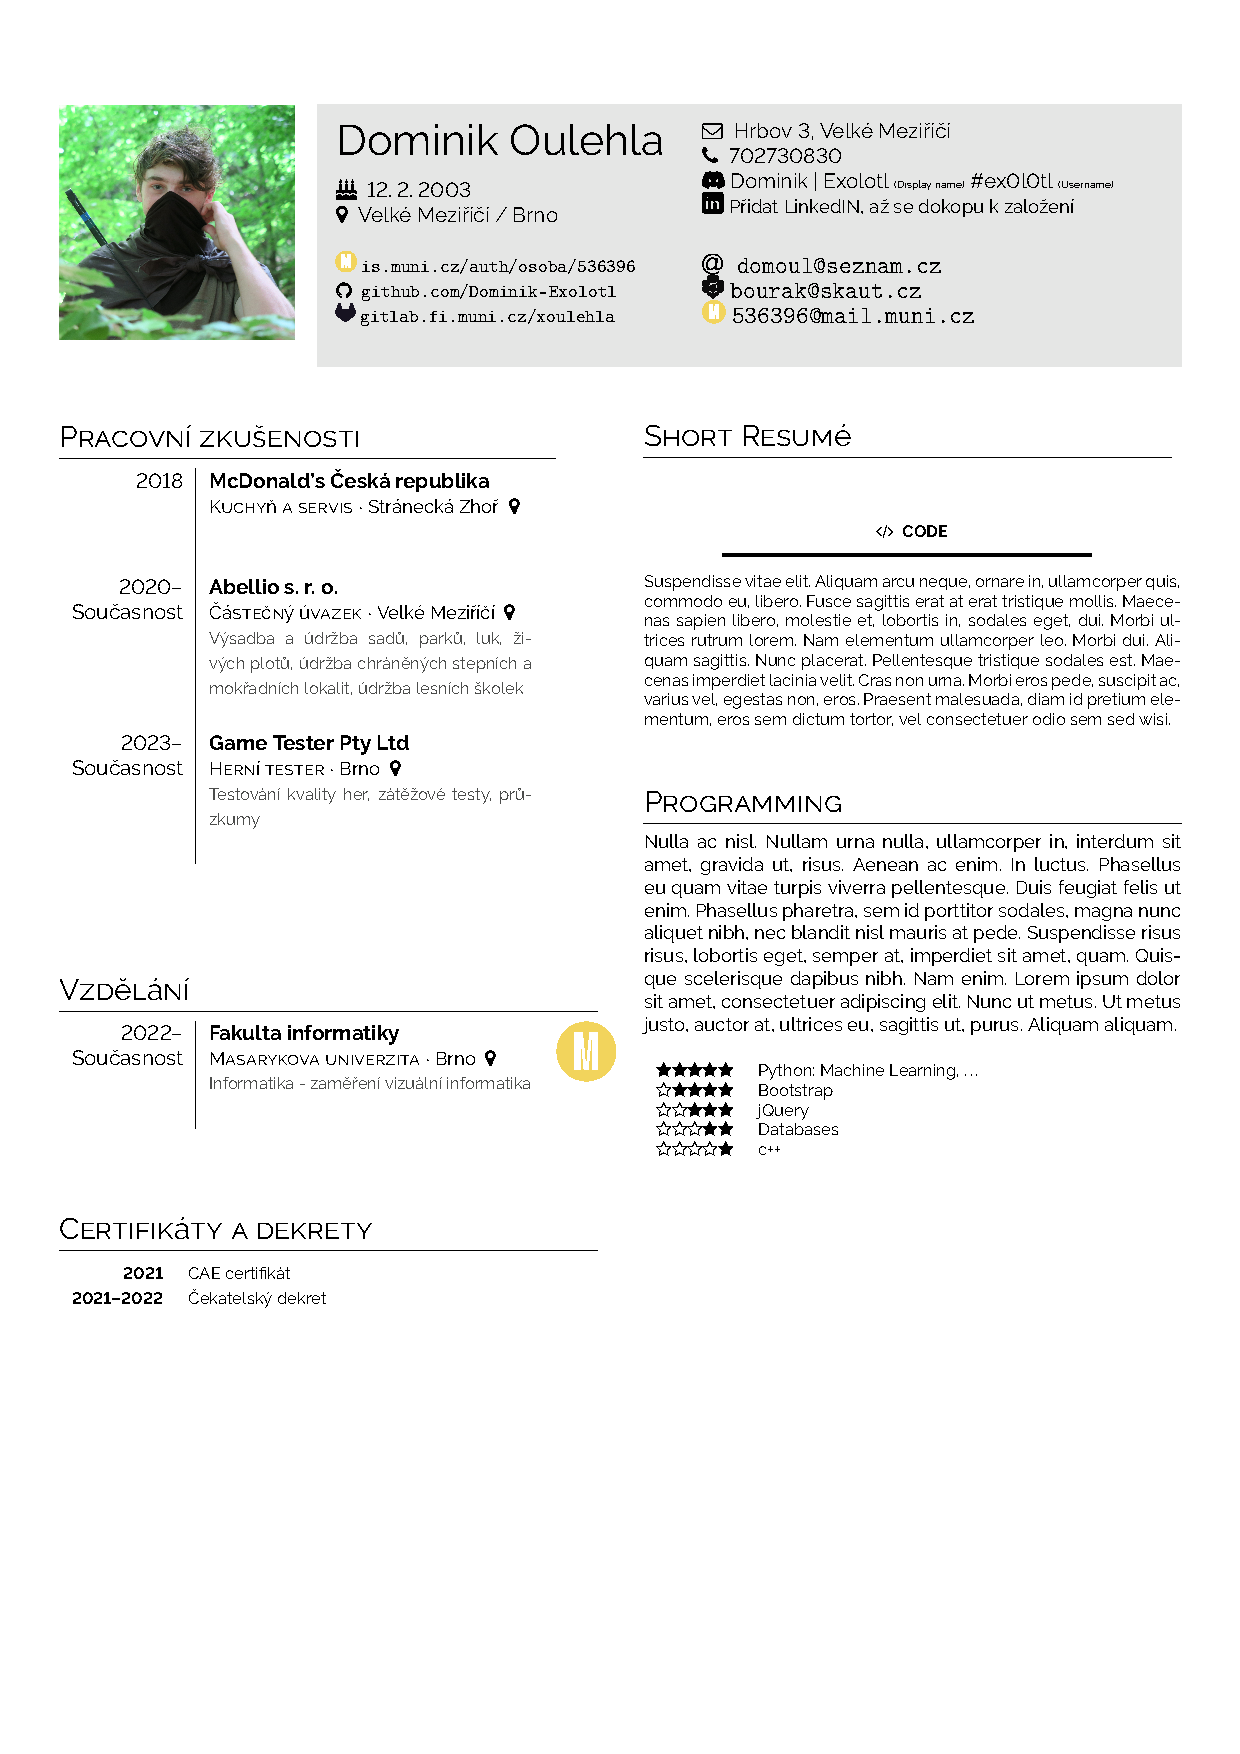
\includepdf[pages=-]{main.pdf}
\directlua{newpax.writenewpax("finals_thesis")}
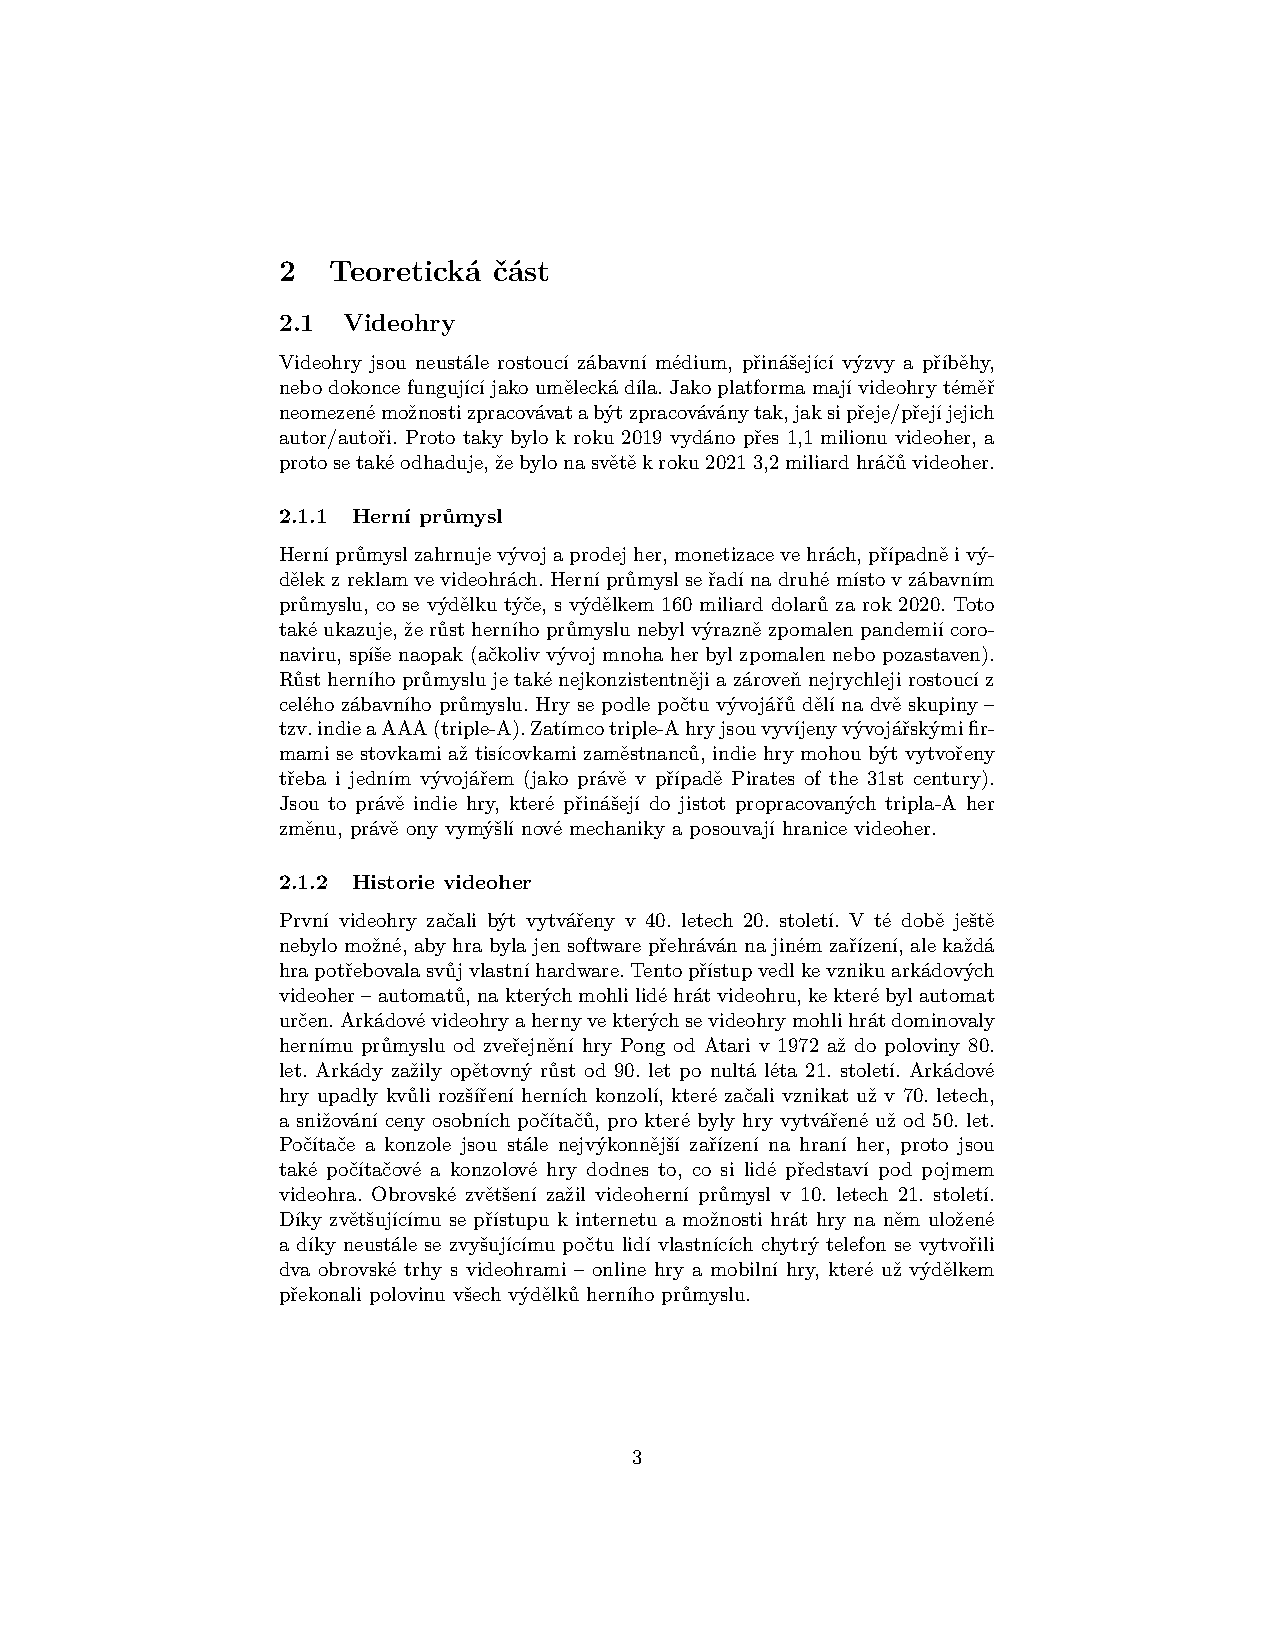
\includepdf[pages=1-3]{finals_thesis.pdf}
\end{document}